\documentclass[a4paper,  11pt]{ctexart}
\usepackage{srcltx,graphicx}
\usepackage{amsmath, amssymb, amsthm}
\usepackage{color}
\usepackage{lscape}
\usepackage{multirow}
\usepackage{psfrag}
\usepackage{diagbox}
\usepackage[hang]{subfigure}
\usepackage{float}
\usepackage[colorlinks,linkcolor=black,anchorcolor=blue,citecolor=green]{hyperref}

\newtheorem{theorem}{Theorem}
\newtheorem{lemma}{Lemma}
\newtheorem{definition}{Definition}
\newtheorem{comment}{Comment}
\newtheorem{conjecture}{Conjecture}

\newcommand\bbR{\mathbb{R}}
\newcommand\bbN{\mathbb{N}}
\newcommand\bbC{\mathbb{C}}
\newcommand\bx{\boldsymbol{x}}
\newcommand\dd{\,\mathrm{d}}

\newcommand\diag{\mathrm{diag}}
\newcommand\tr{\mthrm{tr}}

\setlength{\oddsidemargin}{0cm}
\setlength{\evensidemargin}{0cm}
\setlength{\textwidth}{150mm}
\setlength{\textheight}{230mm}

\newcommand\note[2]{{{\bf #1}\color{red} [ {\it #2} ]}}
%\newcommand\note[2]{{ #1 }} % using this line in the formal version

\newcommand\pd[2]{\dfrac{\partial {#1}}{\partial {#2}}}
\newcommand\od[2]{\dfrac{\dd {#1}}{\dd {#2}}}
\newcommand{\bm}[1]{\mbox{\boldmath{$#1$}}}

\begin{document}
\title{计算系统生物学作业-上机部分}
\author{郑灵超 1601110040}
\maketitle
% \tableofcontents
% \newpage

\section*{4.2}
\subsection*{a}
\begin{figure}[H]
  \centering 
  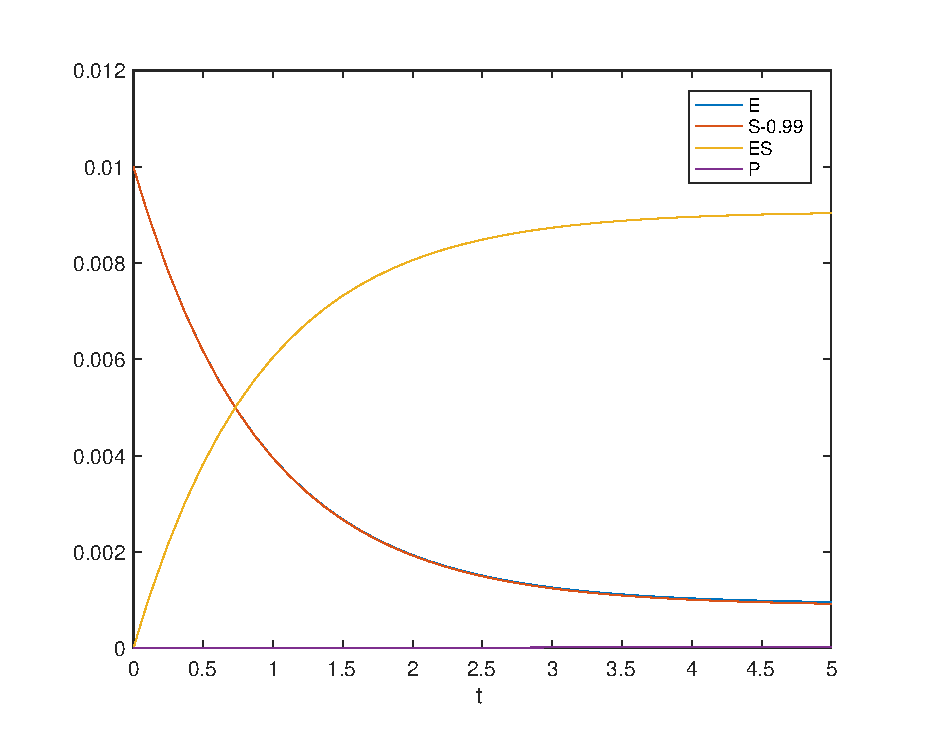
\includegraphics[width=0.9\textwidth]{fig1.eps}
\end{figure}
此处由于$[S]$较大,将$[S]$减去0.99进行比较。
\subsection*{b}
\begin{figure}[H]
  \subfigure[]{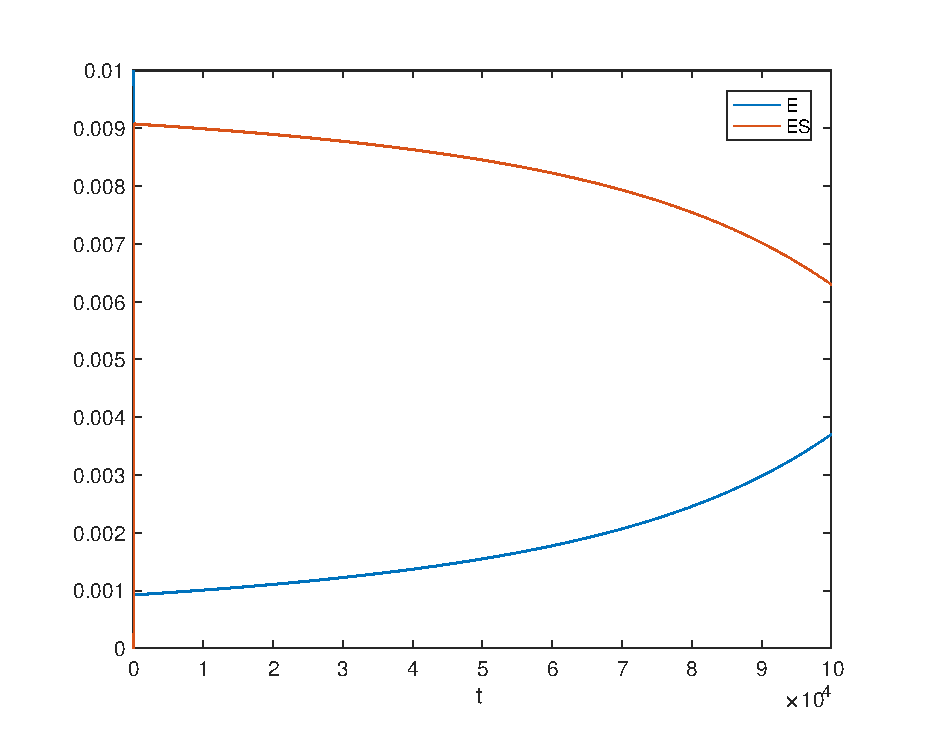
\includegraphics[width=0.45\textwidth]{fig2-1.eps}}
  \subfigure[]{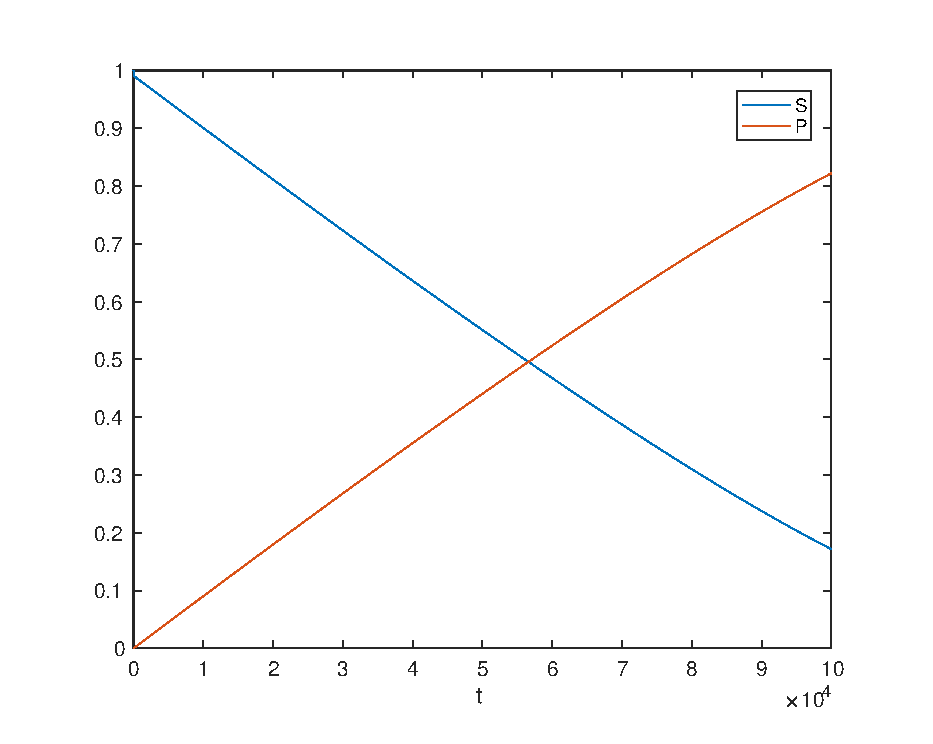
\includegraphics[width=0.45\textwidth]{fig2-2.eps}}
\end{figure}
\subsection*{c and d}
\begin{figure}[H]
  \centering 
  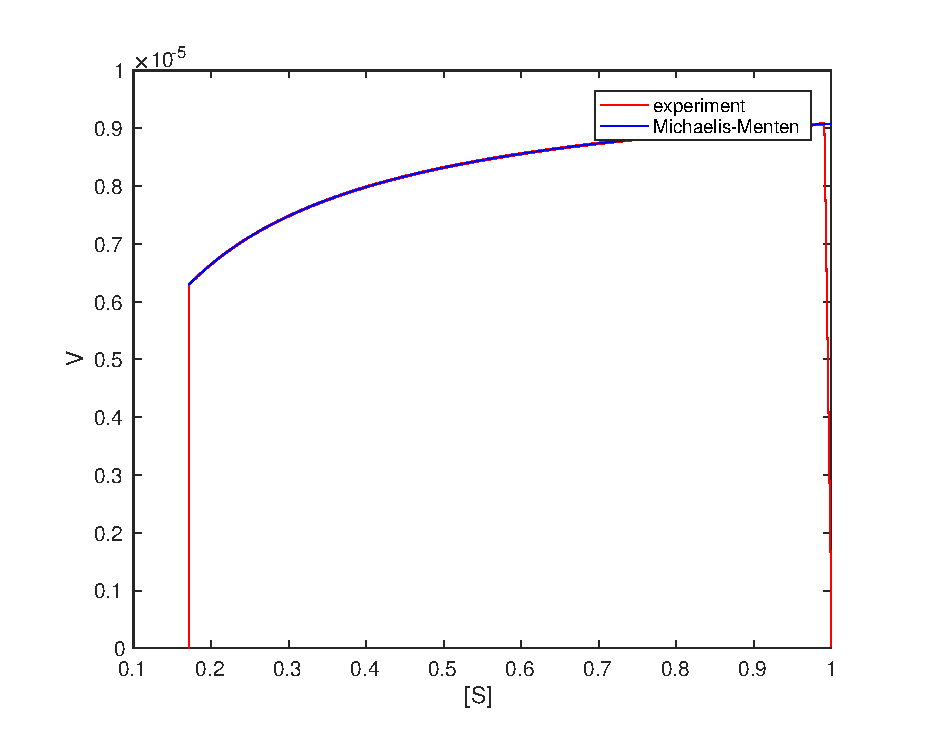
\includegraphics[width=0.9\textwidth]{fig3.eps}
\end{figure}
在$[S]$接近于1时由于实验中$[ES]$很小,二者出现偏差。
\section*{4.3}
\subsection*{a}
\[
V_{max} = k_2E_0, \quad K_m = \frac{k_{-1}+k_2}{k_{+1}}.
\]
\subsection*{b, c, and d}
\begin{figure}[H]
  \centering 
  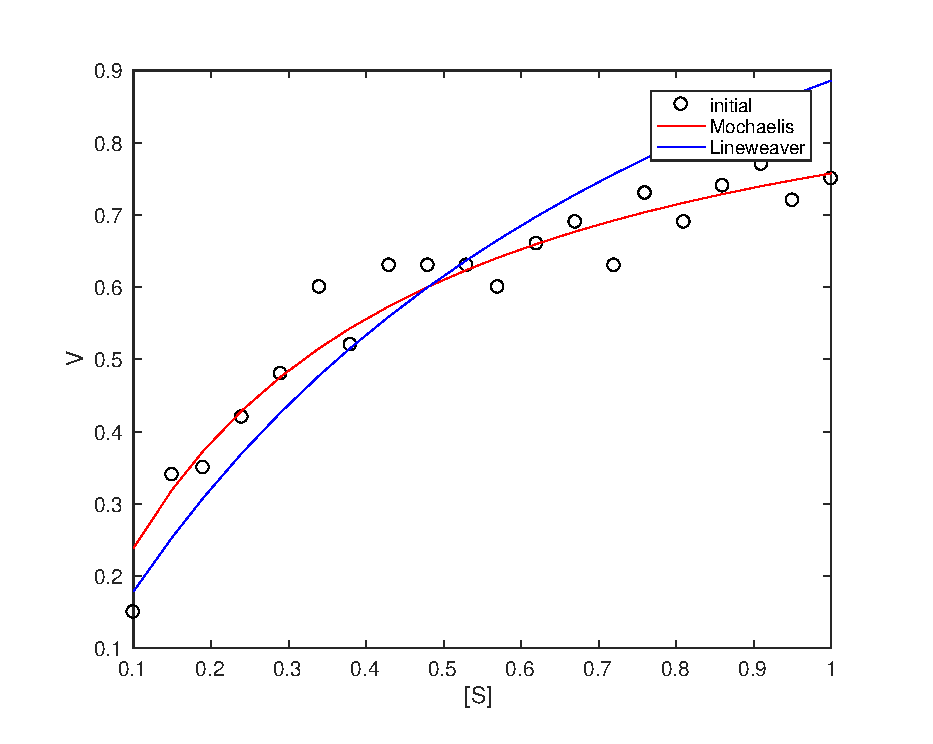
\includegraphics[width=0.9\textwidth]{fig4.eps}
\end{figure}
按照b题方案
\[  
  V_{max} = 0.9986, \quad K_{m} = 0.3181;
\]

按照c题方案
\[  
  V_{max} = 1.5809, \quad K_{m} = 0.7839;
\] 

由于采用模型不同,二者具有较大差距。

\end{document}
